\chapter[Leetcode Algorithms P1-P100]
{Leetcode Algorithms P1-P100
  \label{chP1P100}}
\chaptermark{LC P1-P100}

Notes on LeetCode problems up to 100

%%%%%%%%%%%%%%%%%%%%%%%%%%%%%%%%%%%%%%%%%%%%%%%%%%%%%%%%%%%%%%%%%%%%%%%%%%%%
%%%%%%%%%%%%%%%%%%%%%%%%%%%%%%%%%%%%%%%%%%%%%%%%%%%%%%%%%%%%%%%%%%%%%%%%%%%%
%%%%%%%%%%%%%%%%%%%%%%%%%%%%%%%%%%%%%%%%%%%%%%%%%%%%%%%%%%%%%%%%%%%%%%%%%%%%
%%%%%%%%%%%%%%%%%%%%%%%%%%%%%%%%%%%%%%%%%%%%%%%%%%%%%%%%%%%%%%%%%%%%%%%%%%%%
\section{11: Container With Most Water
  \label{secAlgoP11CntnrWthMstWtr}}

Given n non-negative integers $a_1$, $a_2$, $\ldots$, $a_n$, where each
represents a point at coordinate $(i,a_i)$. $n$ vertical lines are drawn
such that the two endpoints of line $i$ is at $(i,a_i)$ and $(i,0)$. Find
two lines, which together with $x$-axis forms a container, such that the
container contains the most water.

Note: You may not slant the container and $n$ is at least $2$.

\rrsepline{}

\rrheader{Approach \#1 Brute Force [Time Limit Exceeded]}

\noindent{}\textbf{Algorithm}\\
In this case, we will simply consider the area for every possible pair of
the lines and find out the maximum area out of those.
\begin{lstlisting}[style=raycppnewsnippet]
public class Solution {
  public int maxArea(int[] height) 
  {
    int maxarea = 0;
    for (int i = 0; i < height.length; i++)
      for (int j = i + 1; j < height.length; j++)
        maxarea = Math.max(maxarea, Math.min(height[i],
                                             height[j]) * (j - i));
    
    return maxarea;
  }
}
\end{lstlisting}

\noindent{}\textbf{Complexity Analysis}\\
\begin{itemize}[noitemsep,topsep=0pt]
\item Time complexity: $\comBigOh{n^2}$. Calculating areas for all
  $\displaystyle \frac{n(n-1)}{2}$ height pairs.
\item Space complexity: $\comBigOh{1}$. Constant extra space used.
\end{itemize}

Note that we only have to consider $\frac{n(n-1)}{2}$ pairs (to calculate
the areas), since once we've calculated the area for $i$ with $j$, the area
for $j$ with $i$ is the same.  That is, they are symmetric.

\rrheader{Approach \#2 (Two Pointer Approach) [Accepted]}

\noindent{}\textbf{Algorithm}\\
The intuition behind this approach is that the area formed between the lines
will always be limited by the height of the shorter line. Further, the
farther the lines, the more will be the area obtained.

We take two pointers, one at the beginning and one at the end of the array
constituting the length of the lines. Further, we maintain a variable
\ctt{maxarea} to store the maximum area obtained till now. At every step, we
find out the area formed between them, update \ctt{maxarea} and move the
pointer pointing to the \textbf{shorter line} towards the other end by one
step.

The algorithm can be better understood by looking at the example below:
\begin{lstlisting}[style=raygeneric]
1 8 6 2 5 4 8 3 7
\end{lstlisting}

See the gif here:
\url{https://leetcode.com/problems/container-with-most-water/solution}

How this approach works?

Initially we consider the area constituting the exterior most lines. Now, to
maximize the area, we need to consider the area between the lines of larger
lengths. 

\textbf{If we try to move the pointer at the longer line inwards, we won't
gain any increase in area, since it is limited by the shorter line.}
\rrblue{(Think about it, since moving the longer line will reduce the length
  of the base, but the height is still limited by the shorter line.)}

\textbf{But moving the shorter line's pointer could turn out to be
  beneficial, as per the same argument, despite the reduction in the width.}
\rrblue{(Since we may read a line where the height more than offset the
  reduction in width.)} \emph{This is done since a relatively longer line
  obtained by moving the shorter line's pointer might overcome the reduction
  in area caused by the width reduction.}

For further clarification click
here\footnote{\url{https://discuss.leetcode.com/topic/3462/yet-another-way-to-see-what-happens-in-the-o-n-algorithm}}
and for the proof click
here\footnote{\url{https://discuss.leetcode.com/topic/503/anyone-who-has-a-o-n-algorithm/2}}.

I shall cover both now.

\rrsepline{}

The $\comBigOh{n}$ solution with proof by contradiction doesn't look
intuitive enough to me. Before moving on, read the algorithm first if you
don't know it yet.

Here's another way to see what happens in a matrix representation:

Draw a matrix where the row is the first line, and the column is the second
line. For example, say $n=6$.

In the figures below, $x$ means we don't need to compute the volume for that
case: \textbf{(1)} On the diagonal, the two lines are overlapped;
\textbf{(2)} The lower left triangle area of the matrix is symmetric to the
upper right area.

We start by computing the volume at $(1,6)$, denoted by $o$. Now, if the
left line is shorter than the right line, then all the elements left to
$(1,6)$ on the first row have smaller volume \rrblue{(because in those, we
  keep the shorter one still $(i=1)$ but we move the longer one $(j=6)$,
  thus reducing the width)}, so we don't need to compute those cases
(crossed by $-{}-{}-$).
\begin{lstlisting}[style=raygeneric]
  1 2 3 4 5 6
1 x ------- o
2 x x
3 x x x 
4 x x x x
5 x x x x x
6 x x x x x x
\end{lstlisting}
Next we move the left line and compute $(2,6)$. Now if the right line is
shorter, all cases below $(2,6)$ are eliminated. \rrblue{(If the right line
  is shorter, then the same principal applies, there's no point moving the
  left line $i=2$ towards $j=6$, because we just reduce the width without
  being able to increase the max length of the two lines)}
\begin{lstlisting}[style=raygeneric]
  1 2 3 4 5 6
1 x ------- o
2 x x       o
3 x x x     |
4 x x x x   |
5 x x x x x |
6 x x x x x x
\end{lstlisting}
And no matter how this $o$ path goes, we end up only need to find the max
value on this path, which contains $n-1$ cases.
\begin{lstlisting}[style=raygeneric]
  1 2 3 4 5 6
1 x ------- o
2 x x - o o o
3 x x x o | |
4 x x x x | |
5 x x x x x |
6 x x x x x x
\end{lstlisting}
Hope this helps. I feel more comfortable seeing things this way.

Let's code this up.


%%%%%%%%%%%%%%%%%%%%%%%%%%%%%%%%%%%%%%%%%%%%%%%%%%%%%%%%%%%%%%%%%%%%%%%%%%%%
%%%%%%%%%%%%%%%%%%%%%%%%%%%%%%%%%%%%%%%%%%%%%%%%%%%%%%%%%%%%%%%%%%%%%%%%%%%%
%%%%%%%%%%%%%%%%%%%%%%%%%%%%%%%%%%%%%%%%%%%%%%%%%%%%%%%%%%%%%%%%%%%%%%%%%%%%
%%%%%%%%%%%%%%%%%%%%%%%%%%%%%%%%%%%%%%%%%%%%%%%%%%%%%%%%%%%%%%%%%%%%%%%%%%%%
\section{31: Next Permutation
  \label{secAlgoP31NextPermutation}}

Implement next permutation, which rearranges numbers into the
lexicographically next greater permutation of numbers.

If such arrangement is not possible, it must rearrange it as the lowest
possible order (ie, sorted in ascending order).

The replacement must be in-place, do not allocate extra memory.

Here are some examples. Inputs are in the left-hand column and its
corresponding outputs are in the right-hand column.
\begin{lstlisting}[style=raygeneric]
1,2,3 -> 1,3,2
3,2,1 -> 1,2,3
1,1,5 -> 1,5,1
\end{lstlisting}

\rrsepline{}

\rrheader{Approach \#2 Single Pass Approach [Accepted]}

First, we observe that for any given sequence that is in descending order,
no next larger permutation is possible. For example, no next permutation is
possible for the following array: 
\begin{lstlisting}[style=raygeneric]
9, 5, 4, 3, 1
\end{lstlisting}
We need to find the first pair of two successive numbers \ctt{a[i-1]} and
\ctt{a[i]}, from the right, which satisfy \ctt{a[i]} > \ctt{a[i-1]}. 
E.g. if we have
\begin{lstlisting}[style=raygeneric]
      i-1  i
9, 5, 3,   4, 1
\end{lstlisting}
then we can form a greater permutation since $a[i]=4>3=a[i-1]$.

Now, no rearrangements to the right of \ctt{a[i-1]} can create a larger
permutation \rrhl{since that subarray consists of numbers in descending
  order.} (See the above example.) Thus, we need to rearrange the numbers to
the right of \ctt{a[i-1]} including itself.

Now, what kind of rearrangement will produce the next larger number? We want
to create the permutation just larger than the current one. Therefore, we
need to replace the number \ctt{a[i-1]} with the number which is \rrhl{just}
larger than itself among the numbers lying to its right section, say
\ctt{a[j]}.

\begin{figure}
\centering
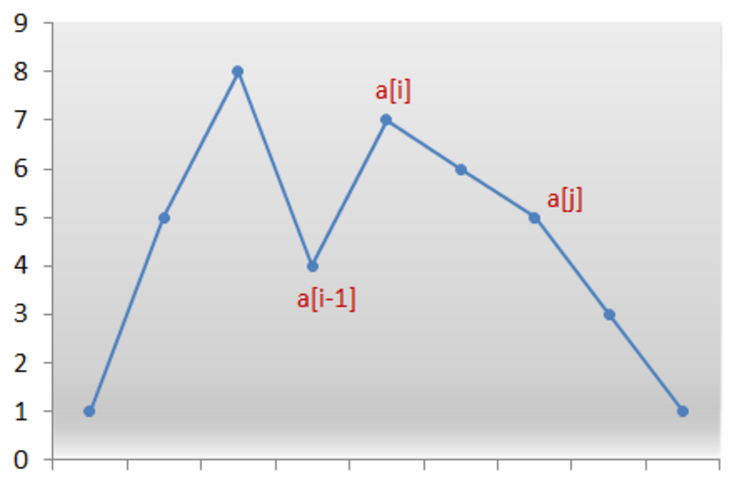
\includegraphics[width=0.7\textwidth]{Images/figP31NextPermutation}
\label{figP31NextPermutation}
\end{figure}

We swap the numbers \ctt{a[i-1]} and \ctt{a[j]}. We now have the correct
number at index $i-1$. But still the current permutation isn't the
permutation that we are looking for. We need the \textbf{smallest
  permutation} that
can be formed by using the numbers only to the right of \ctt{a[i-1]}.
Therefore, \rrhl{we need to place those numbers in ascending order to get their
smallest permutation.}

\rrhl{REMEMBER THAT ASCENDING ORDER = SMALLEST, DESCENDING = LARGEST.} Think
of it in terms of normal numbers, 12345 is smaller than 54321.

But, recall that while scanning the numbers from the right, we simply kept
decrementing the index until we found the pair \ctt{a[i-1]} and \ctt{a[i]}
where, \ctt{a[i]} > \ctt{a[i-1]}. Thus, all numbers to the right of
\ctt{a[i-1]} \rrhl{were already sorted in descending order}. Furthermore,
swapping \ctt{a[i-1]} and \ctt{a[j]} didn't change that order. Therefore, we
simply need to reverse the numbers following \ctt{a[i-1]} to get the next
smallest lexicographic permutation.

The following animation will make things clearer: see the gif in
\url{https://leetcode.com/problems/next-permutation/solution/}




%%%%%%%%%%%%%%%%%%%%%%%%%%%%%%%%%%%%%%%%%%%%%%%%%%%%%%%%%%%%%%%%%%%%%%%%%%%%
%%%%%%%%%%%%%%%%%%%%%%%%%%%%%%%%%%%%%%%%%%%%%%%%%%%%%%%%%%%%%%%%%%%%%%%%%%%%
%%%%%%%%%%%%%%%%%%%%%%%%%%%%%%%%%%%%%%%%%%%%%%%%%%%%%%%%%%%%%%%%%%%%%%%%%%%%
\subsection{GFG: Write a program to print all permutations of a given string
  \label{secGFGWrtAPrgrmTPrntAllPrmttnsOfAGvnStrng}}

\rrblue{I have decided to learn all about permutation algorithm before I
  tackle the above problem.}

\noindent{}\textbf{Diff: 3.5}

A permutation, also called an ``arrangement number'' or ``order,'' is a 
rearrangement of the elements of an ordered list $S$ into a one-to-one 
correspondence with $S$ itself. A string of length $n$ has $n!$ permutation.
Source: Mathword(\url{http://mathworld.wolfram.com/Permutation.html})

Below are the permutations of string ABC.
\begin{lstlisting}[style=raygeneric]
ABC ACB BAC BCA CBA CAB
\end{lstlisting}

\textbf{\rrgreen{Recommended: Please solve it on ``PRACTICE'' first, before
    moving on to the solution.}}

Here is a solution that is used as a basis in backtracking.

\begin{figure}
\centering
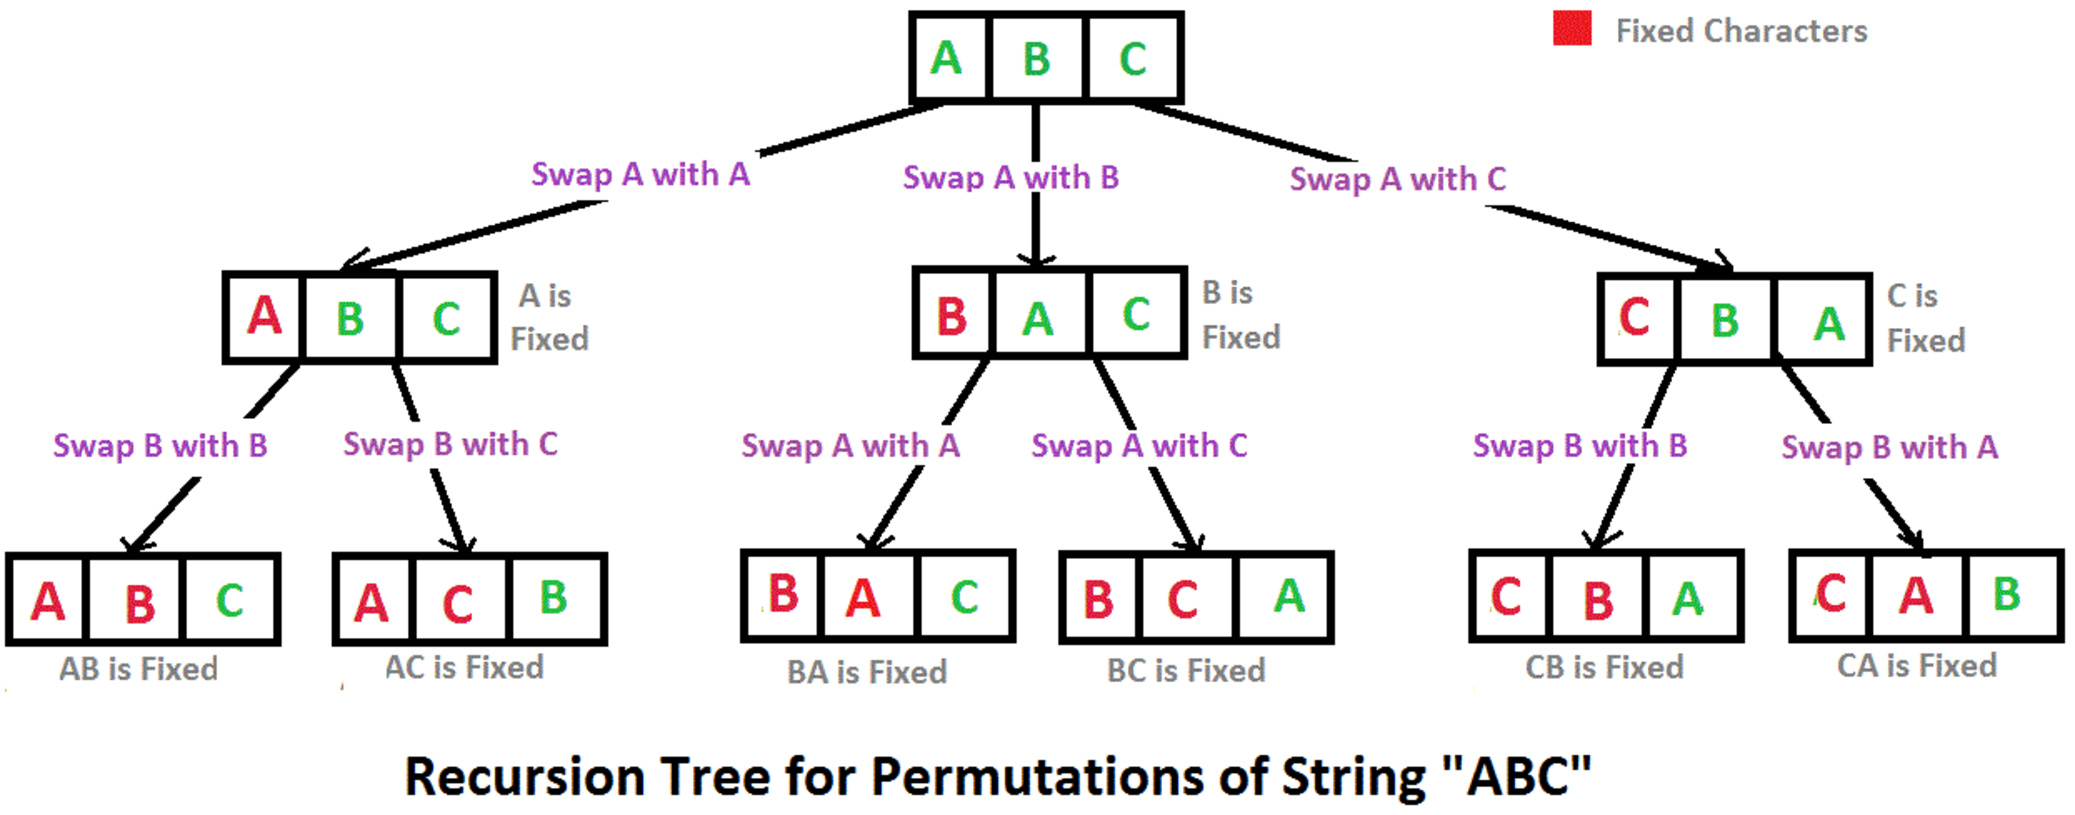
\includegraphics[width=0.7\textwidth]{Images/figGFGNewPermutation}
\label{figGFGNewPermutation}
\end{figure}

\qasepline{}

\begin{enumerate}[label=\textbf{\arabic*.},noitemsep,topsep=0pt]
\item For the first character, we have three choices, A, B and C.
\item Once we have chosen one, then we have 2 choices for the next
  character.
\item For the last character, there is only one choice.
\end{enumerate}

Say we have an array with indices $[0..n-1]$, one way to achieve this is to
do
\begin{lstlisting}[style=pseudostyle,numbers=none]
[0..i..n-1], let 0..i-1 be fixed (already permuted).
for j=i..n-1
  swap(i,j)
  recur (i+1)
\end{lstlisting}

Something like that.

I coded it up: \path{31\_NextPermutation/rrrAllPermutation.cpp}

\noindent{}\textbf{Algorithm Paradigm:} Backtracking\\

\noindent{}\textbf{Time Complexity:} $\comBigOh{n*n!}$: Note that there are
$n!$ permutations and it requires $\comBigOh{n}$ time to print a
permutation.

Note : The above solution prints duplicate permutations if there are
repeating characters in input string. Please see below link for a solution
that prints only distinct permutations even if there are duplicates in
input.

%%%%%%%%%%%%%%%%%%%%%%%%%%%%%%%%%%%%%%%%%%%%%%%%%%%%%%%%%%%%%%%%%%%%%%%%%%%%
%%%%%%%%%%%%%%%%%%%%%%%%%%%%%%%%%%%%%%%%%%%%%%%%%%%%%%%%%%%%%%%%%%%%%%%%%%%%
%%%%%%%%%%%%%%%%%%%%%%%%%%%%%%%%%%%%%%%%%%%%%%%%%%%%%%%%%%%%%%%%%%%%%%%%%%%%
\subsection{GFG: Print all distinct permutations of a given string with duplicates
  \label{secGFGPrntAllDstnctPrmttnsOfAGvnStrngWthDuplcts}}

\noindent{}\textbf{Diff: 4.2}

RRR toread.

Given a string that may contain duplicates, write a function to print all
permutations of given string such that no permutation is repeated in output.

Examples:
\begin{lstlisting}[style=raygeneric]
Input:  str[] = "AB"
Output: AB BA

Input:  str[] = "AA"
Output: AA

Input:  str[] = "ABC"
Output: ABC ACB BAC BCA CBA CAB

Input:  str[] = "ABA"
Output: ABA AAB BAA

Input:  str[] = "ABCA"
Output: AABC AACB ABAC ABCA ACBA ACAB BAAC BACA 
        BCAA CABA CAAB CBAA
\end{lstlisting}
We have discussed an algorithm to print all permutations in below post. It
is strongly recommended to refer below post as a prerequisite of this post.

Write a C program to print all permutations of a given string
(\cref{secGFGWrtAPrgrmTPrntAllPrmttnsOfAGvnStrng}).

The algorithm discussed on above link doesn't handle duplicates.

\begin{lstlisting}[style=raycppnewsnippet]
// Program to print all permutations of a string in sorted order.
#include <stdio.h>
#include <stdlib.h>
#include <string.h>
 
/* Following function is needed for library function qsort(). */
int compare(const void *a, const void * b)
{
  return ( *(char *)a - *(char *)b );
}
 
// A utility function two swap two characters a and b
void swap(char* a, char* b)
{
  char t = *a;
  *a = *b;
  *b = t;
}
 
// This function finds the index of the smallest character
// which is greater than 'first' and is present in str[l..h]
int findCeil(char str[], char first, int l, int h)
{
    // initialize index of ceiling element
    int ceilIndex = l;
 
    // Now iterate through rest of the elements and find
    // the smallest character greater than 'first'
    for (int i = l+1; i <= h; i++)
        if (str[i] > first && str[i] < str[ceilIndex])
            ceilIndex = i;
 
    return ceilIndex;
}

// Print all permutations of str in sorted order
void sortedPermutations(char str[])
{
  // Get size of string
  int size = strlen(str);
 
  // Sort the string in increasing order
  qsort(str, size, sizeof( str[0] ), compare);
 
  // Print permutations one by one
  bool isFinished = false;
  while (!isFinished)
  {
    // print this permutation
    static int x = 1;
    printf("%d  %s \n", x++, str);
 
    // Find the rightmost character which is smaller than its next
    // character. Let us call it 'first char'
    int i;
    for (i = size - 2; i >= 0; --i)
      if (str[i] < str[i+1])
        break;
 
    // If there is no such chracter, all are sorted in decreasing order,
    // means we just printed the last permutation and we are done.
    if (i == -1)
      isFinished = true;
    else
    {
      // Find the ceil of 'first char' in right of first character.
      // Ceil of a character is the smallest character greater than it
      int ceilIndex = findCeil(str, str[i], i + 1, size - 1);
 
      // Swap first and second characters
      swap(&str[i], &str[ceilIndex]);
 
      // Sort the string on right of 'first char'
      qsort(str + i + 1, size - i - 1, sizeof(str[0]), compare);
    }
  }
}
 
// Driver program to test above function
int main()
{
  char str[] = "ACBC";
  sortedPermutations( str );
  return 0;
}
\end{lstlisting}
Output:
\begin{lstlisting}[style=rayio]
1  ABCC
2  ACBC
3  ACCB
4  BACC
5  BCAC
6  BCCA
7  CABC
8  CACB
9  CBAC
10  CBCA
11  CCAB
12  CCBA
\end{lstlisting}
The above code is taken from a comment below by Mr. Lazy.
\begin{itemize}[noitemsep,topsep=0pt]
\item Time Complexity: $\comBigOh{n2\times n!}$
\item Auxiliary Space: $\comBigOh{1}$.
\end{itemize}

%%%%%%%%%%%%%%%%%%%%%%%%%%%%%%%%%%%%%%%%%%%%%%%%%%%%%%%%%%%%%%%%%%%%%%%%%%%%
%%%%%%%%%%%%%%%%%%%%%%%%%%%%%%%%%%%%%%%%%%%%%%%%%%%%%%%%%%%%%%%%%%%%%%%%%%%%
%%%%%%%%%%%%%%%%%%%%%%%%%%%%%%%%%%%%%%%%%%%%%%%%%%%%%%%%%%%%%%%%%%%%%%%%%%%%
\subsection{GFG: Permutations of a given string using STL
  \label{secGFGPrntAllDstnctPrmttnsOfAGvnStrngWthDuplcts}}

\noindent{}\textbf{Diff: 3.6}

\url{https://www.geeksforgeeks.org/permutations-of-a-given-string-using-stl}

A permutation, also called an ``arrangement number'' or ``order'', is a 
rearrangement of the elements of an ordered list $S$ into a one-to-one 
correspondence with $S$ itself. A string of length $n$ has $n!$ permutation.

Below are the permutations of string $ABC$.
$ABC$ $ACB$ $BAC$ $BCA$ $CBA$ $CAB$
We have discussed C implementation to print all permutations of a given
string using backtracking here. In this post, C++ implementation using STL
is discussed.

\rrheader{Method 1 (Using rotate())}

\ctt{std::rotate} function rotates elements of a vector/string such that the
passed middle element becomes first. For example, if we call \ctt{rotate}
for ``\ctt{ABCD}'' with middle as second element, the string becomes
``\ctt{BCDA}'' and if we again call rotate with middle as second element,
the string becomes ``\ctt{CDAB}''.  Refer this for a sample program.

\begin{figure}
\centering
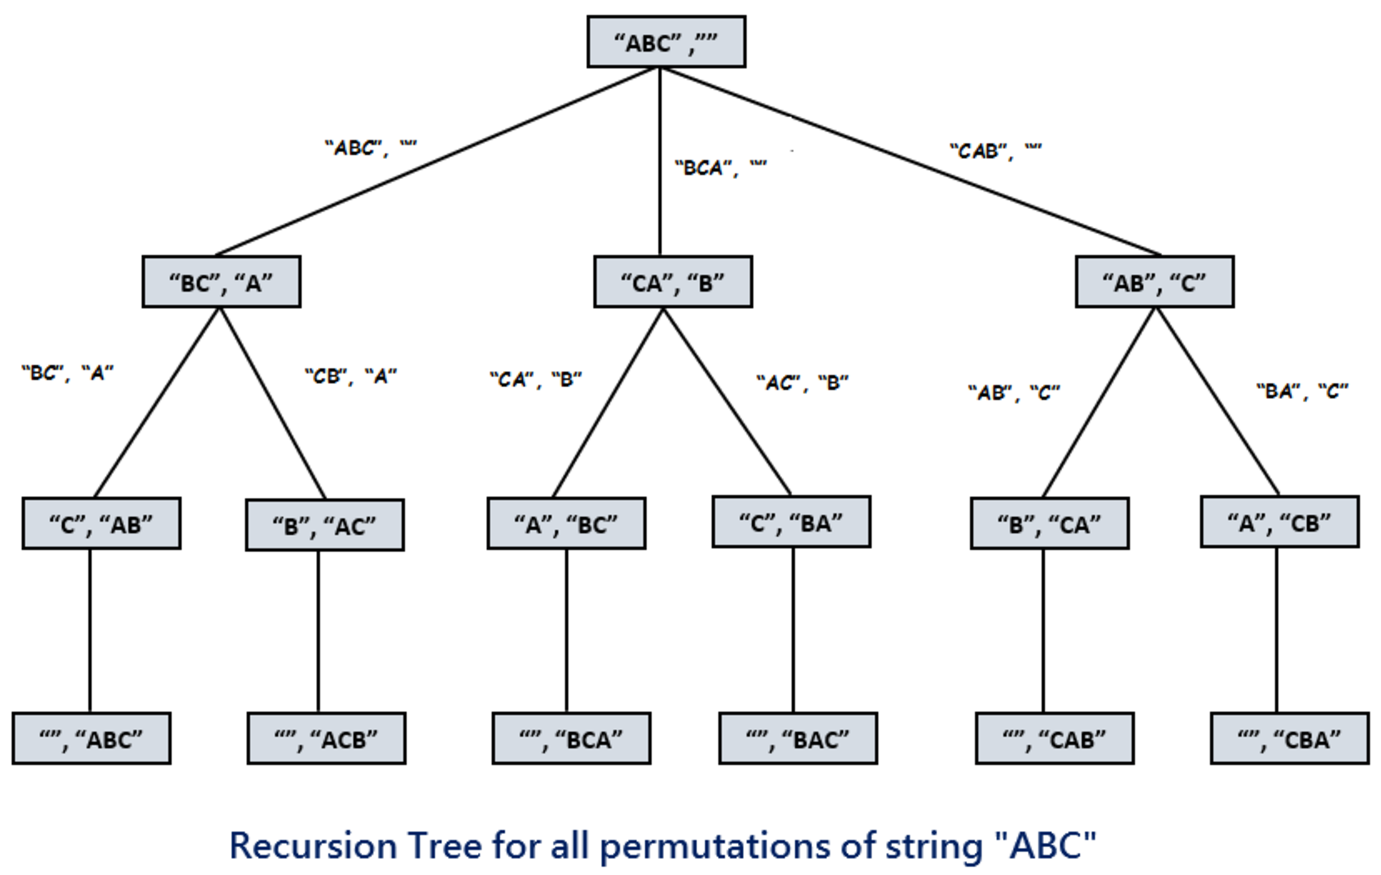
\includegraphics[width=1\textwidth]{Images/figGFGPermuteRotateRecur}
\label{figGFGPermuteRotateRecur}
\end{figure}

Below is C++ implementation.
\begin{lstlisting}[style=raycppnewsnippet]
// C++ program to print all permutations with
// duplicates allowed using rotate() in STL
#include <bits/stdc++.h>
using namespace std;
 
// Function to print permutations of string str,
// out is used to store permutations one by one
void permute(string str, string out)
{
  // When size of str becomes 0, out has a
  // permutation (length of out is n)
  if (str.size() == 0)
  {
    cout << out << endl;
    return;
  }
 
  // One by one move all characters at
  // the BEGINNING of out (or result)
  for (int i = 0; i < str.size(); i++)
  {
    // Remove first character from str and
    // add it to out
    permute(str.substr(1), out + str[0]);
 
    // Rotate string in a way second character
    // moves to the beginning.
    rotate(str.begin(), str.begin() + 1, str.end());
  }
}
 
// Driver code
int main()
{
  string str = "ABC";
  permute(str, "");
  return 0;
}
\end{lstlisting}


%%%%%%%%%%%%%%%%%%%%%%%%%%%%%%%%%%%%%%%%%%%%%%%%%%%%%%%%%%%%%%%%%%%%%%%%%%%%
%%%%%%%%%%%%%%%%%%%%%%%%%%%%%%%%%%%%%%%%%%%%%%%%%%%%%%%%%%%%%%%%%%%%%%%%%%%%
%%%%%%%%%%%%%%%%%%%%%%%%%%%%%%%%%%%%%%%%%%%%%%%%%%%%%%%%%%%%%%%%%%%%%%%%%%%%
%%%%%%%%%%%%%%%%%%%%%%%%%%%%%%%%%%%%%%%%%%%%%%%%%%%%%%%%%%%%%%%%%%%%%%%%%%%%
\section{33: Search in Rotated Sorted Array
  \label{secAlgoP33SearchInRotSortArry}}

Suppose an array sorted in ascending order is rotated at some pivot unknown
to you beforehand.

(i.e., \ctt{0 1 2 4 5 6 7} might become \ctt{4 5 6 7 0 1 2}).

You are given a target value to search. If found in the array return its
index, otherwise return \ctt{-1}.

You may assume no duplicate exists in the array.

\rrsepline{}

Let's work with an example:
\begin{lstlisting}[style=raycppnewsnippet]
4 5 6 7 8 9 0 1 2, size = 9
\end{lstlisting}
Let's say we want to find \ctt{1}. What information do we have? We have the
two end points, 4 and 2. If \ctt{left} > \ctt{right} then we know that it is
shifted.

So what we can do is a modified binary search.
\begin{enumerate}[label=\textbf{\arabic*.},noitemsep,topsep=0pt]
\item Split the array into\\
  $[leftlo = 0..size / 2 = lefthi]$  $[rightlo=size/2+1..size-1=righthi]$.
\item Find out which side is sorted and test the sorted side first.

\end{enumerate}




%%%%%%%%%%%%%%%%%%%%%%%%%%%%%%%%%%%%%%%%%%%%%%%%%%%%%%%%%%%%%%%%%%%%%%%%%%%%
%%%%%%%%%%%%%%%%%%%%%%%%%%%%%%%%%%%%%%%%%%%%%%%%%%%%%%%%%%%%%%%%%%%%%%%%%%%%
%%%%%%%%%%%%%%%%%%%%%%%%%%%%%%%%%%%%%%%%%%%%%%%%%%%%%%%%%%%%%%%%%%%%%%%%%%%%
%%%%%%%%%%%%%%%%%%%%%%%%%%%%%%%%%%%%%%%%%%%%%%%%%%%%%%%%%%%%%%%%%%%%%%%%%%%%
\section{No: Name
  \label{secAlgoPNumName}}



\rrsepline{}











































